\chapter{More Functions}

\begin{corollary}
    [Functions of the Co-domain]
    \[
        f:A \to B \qquad g: B \to C
    \]
    % draw the set diagrams
    \begin{figure}
        \centering
        \begin{tikzpicture}
            % Define the sets
            \node (A1) at (0,3) {$A$};
            \node (A2) at (0,2) {$a_1$};
            \node (A3) at (0,1) {$a_2$};
            \node (A4) at (0,0) {$a_3$};
            \node (A5) at (0,-1) {$a_4$};

            \node (B1) at (4,3) {$B$};
            \node (B2) at (4,2) {$b_1$};
            \node (B3) at (4,1) {$b_2$};
            \node (B4) at (4,0) {$b_3$};
            \node (B5) at (4,-1) {$b_4$};

            \node (C1) at (8,3) {$C$};
            \node (C2) at (8,2) {$c_1$};
            \node (C3) at (8,1) {$c_2$};
            \node (C4) at (8,0) {$c_3$};
            \node (C5) at (8,-1) {$c_4$};

            % Draw arrows
            \draw[->] (A2) -- (B2);
            \draw[->] (A3) -- (B3);
            \draw[->] (A4) -- (B4);
            \draw[->] (A5) -- (B5);

            \draw[->] (B2) -- (C2);
            \draw[->] (B3) -- (C3);
            \draw[->] (B4) -- (C4);
            \draw[->] (B5) -- (C5);

            % Draw sets
            \draw[dashed] (-0.5,3.5) rectangle (0.5,-1.5);
            \draw[dashed] (3.5,3.5) rectangle (4.5,-1.5);
            \draw[dashed] (7.5,3.5) rectangle (8.5,-1.5);
        \end{tikzpicture}
        \caption{Functions of the Co-domain}
        \label{fig:co-domain}

    \end{figure}
\end{corollary}

\begin{definition}
    [Powers of Sets]
    The set of all functions from $A$ to $B$ is denoted by $B^A$.
\end{definition}

\begin{example}
    [Powers of Sets]
    if $A = \{1, 2\}$ and $B = \{x,y,z\}$, then $B^A$ has $3^2 = 9$ elements.
\end{example}

\begin{example}
    [Powers of Sets 2]
    \begin{align*}
        f & = \begin{matrix}
                  1    & 2    \\
                  f(1) & f(2)
              \end{matrix} \\ B^A &= \{ \begin{matrix}
            1 & 2 \\
            x & x
        \end{matrix}, & \begin{matrix}
            1 & 2 \\
            x & y
        \end{matrix}, & \begin{matrix}
            1 & 2 \\
            x & z
        \end{matrix} \\ \begin{matrix}
            1 & 2 \\
            y & x
        \end{matrix} & \begin{matrix}
            1 & 2 \\
            y & y
        \end{matrix} & \begin{matrix}
            1 & 2 \\
            y & z
        \end{matrix} \\ \begin{matrix}
            1 & 2 \\
            z & x
        \end{matrix} & \begin{matrix}
            1 & 2 \\
            z & y
        \end{matrix} & \begin{matrix}
            1 & 2 \\
            z & z
        \end{matrix}\}
    \end{align*}
\end{example}

\section{The Complex Exponential Function}

\begin{definition}
    [The Complex Exponential Function]
    \begin{align*}
        \exp : \mathbb{C} & \to \mathbb{C} \quad \text{via}                                                                         \\
        z                 & \mapsto \exp(z) = 1 + z + \frac{z^2}{2!} + \frac{z^3}{3!} + \cdots = \sum_{n=0}^{\infty} \frac{z^n}{n!}
    \end{align*}
    $exp$ is an entire function, so the taylor series converges for all $z \in \mathbb{C}$.
\end{definition}
\begin{proof}
    Apply the ratio test to prove that the series converges at all $z \in \mathbb{C}$.
\end{proof}

\begin{example}
    [Euler's Relation]
    Say $z = j\theta | \theta \in \mathbb{R}$
    \begin{align*}
        \exp(j\theta) & = 1 + j\theta - \frac{\theta^2}{2!} - j\frac{\theta^3}{3!} + \frac{\theta^4}{4!} + j\frac{\theta^5}{5!} + \cdots            \\
                      & = (1 - \frac{\theta^2}{2!} + \frac{\theta^4}{4!} - \cdots) + j(\theta - \frac{\theta^3}{3!} + \frac{\theta^5}{5!} - \cdots) \\
                      & = \cos(\theta) + j\sin(\theta)
    \end{align*}

\end{example}

\begin{definition}
    [Principle Argument]
    The principle argument of $z \in \mathbb{C}$ is denoted by $\arg(z)$ and is defined as the angle between the positive real axis and the line segment from the origin to $z$.
    \[
        -\pi < \arg(z) = \theta \leq \pi \quad \text{where} \quad \theta = |z| \exp(j\theta)
    \]
\end{definition}

\begin{definition}
    [Polar form Conjugation]
    \[
        \overline{z} = |z| \exp(-j\theta) = x - jy \quad \text{where} \quad z = x + jy
    \]
\end{definition}

\section{Signals}
\subsection*{Four Types of Signals}
\begin{enumerate}
    \item Discrete-Time Signals
    \item \begin{enumerate}
              \item $\mathbb{R}^{\mathbb{Z}}$ Real-valued signals
              \item $\mathbb{C}^{\mathbb{Z}}$ Complex-valued signals
          \end{enumerate}
    \item Continuous-Time Signals
    \item \begin{enumerate}
              \item $\mathbb{R}^{\mathbb{R}}$ Real-valued signals
              \item $\mathbb{C}^{\mathbb{R}}$ Complex-valued signals
          \end{enumerate}
\end{enumerate}

\begin{example}
    [Real-Valued Signals]
    \[x : \mathbb{R} \to \mathbb{R} \qquad\qquad y : \mathbb{Z} \to \mathbb{R}\]
    \begin{figure}
        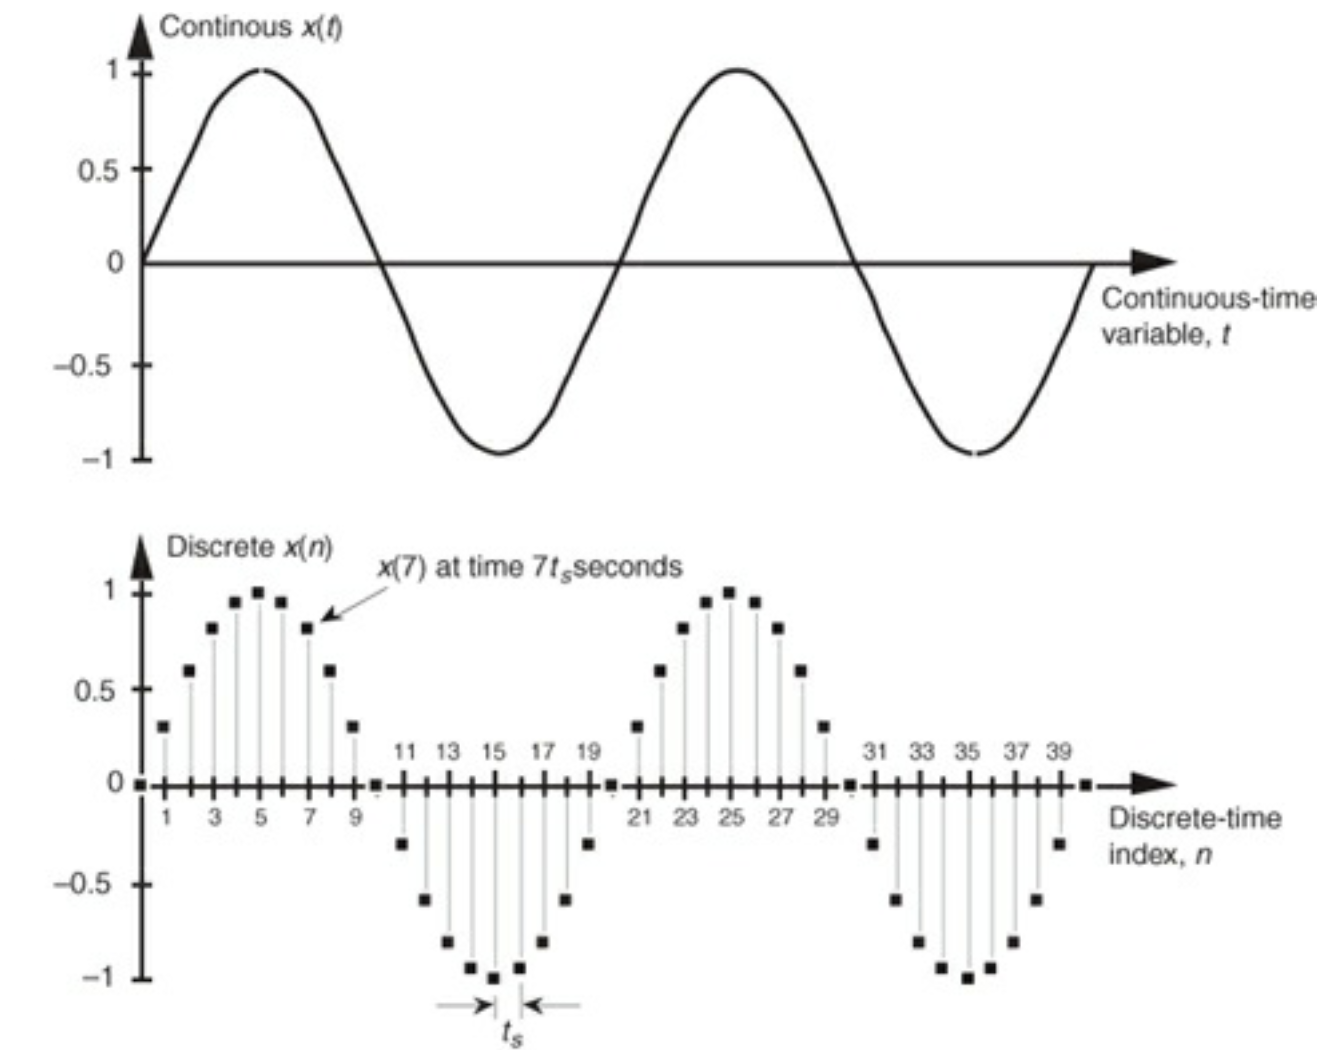
\includegraphics[scale=1]{./LECTURE_2/audio_5.png}
        \caption{Real-Valued Signals}
    \end{figure}
    \[x(t) \qquad \qquad x[t]\]
\end{example}
\begin{definition}
    [Support]
    The \textit{support} of a nonzero signl $x \in \mathbb{C}^\mathbb{R}$ is the smallest interval $[a,b]$ such that $x(t) = 0$ for all $t \notin [a,b]$. \\
    Essentially, the support is the set of all $t$ such that $x(t) \neq 0$.
    IMAGE
\end{definition}

\begin{definition}
    [Energy]
    The \textit{energy} of a signal $x \in \mathbb{C}^\mathbb{R}$ is defined as
    \[
        E_x = \int_{-\infty}^{\infty} |x(t)|^2 dt
    \]
    If $x \in \mathbb{C}^\mathbb{R}$
    \[
        E_x = \int_{t=-\infty}^{\infty} |x(t)|^2
    \]
\end{definition}

\begin{definition}
    [Average Power]
    The \textit{average power} of a signal $x \in \mathbb{C}^\mathbb{R}$ is defined as
    \[
        P_x = \lim_{T \to \infty} \frac{1}{2T} \int_{-T}^{T} |x(t)|^2 dt
    \]
\end{definition}


% simple circuit with voltage source and resistor
% \begin{figure}
%     \centering
%     \begin{circuitikz}
%         \draw (0,0) to[V, v=$V_s$] (0,2) to[R, l=$R$] (2,2) to[short] (2,0) to[short] (0,0);
%     \end{circuitikz}
%     \caption{Simple Circuit}
%     \label{fig:simple-circuit}
% \end{figure}

\begin{remark}
    Homework is assigned!
\end{remark}